Um die sehr unterschiedlichen Implementierungen miteinander vergleichbar zu machen, werden Eigenschaften als Kriterien benötigt. Idealer Weise sind sie auf jede einzelne zutreffen und relevant für den wirtschaftlichen Betrieb einer \gls{BC}.
%~ Diese Kriterien auch sollen relevant für den Anwendungsfall, eventuelle Einschränkungen und die Notwendigkeit zur .
Die Wertung soll klar von geringer Zielerfüllung zur höheren erkennbar sein.


%%
\section{Grundlegendes zur Informationstechnologie}\label{krit:it}
%%

Grundsätzlich treffen die folgenden Annahmen auch auf andere Bereiche innerhalb der Softwaretechnologie zu.
Allerdings ist die Bedeutung erst seit der Erfindung des Personal Computers und Zugang zum Internet für große Bevölkerungsteile durchsetzbar.
Gerade diese Parallele der Entwicklung des Internets zu dem Wandel den auch die \gls{BCT} bringen kann, ist der Grund hier auf eine Verbesserung des Zugangs und eine erneute Dezentralisierung abzuzielen.
Aber nicht nur für den direkten Kundenkontakt entworfene oder in der Interaktion mit anderen Unternehmen befindliche IT-Systeme profitieren von der neuen Offenheit und Dezentralisierung. Auch die IT-Architektur innerhalb eines Unternehmens wird gestärkt wenn zentrale Schwachpunkte vermieden werden. 

%
\subsection{Offener Standard}\label{krit:openstandard}

Die Standardisierung einer Blockchain ist ein wesentlicher Bestandteil zur Sicherung der beabsichtigten Anwendungsfälle.
Sowohl die Dokumentation bisher getroffener Entscheidungen als auch der Prozess für neue Entscheidungen sollten daher standardisiert sein um beurteilt oder in Zukunft an die Erfordernisse angepasst werden zu können.

Über einzelne \gls{BCI} hinweg bringt die Standardisierung auch Austauschmöglichkeiten wie \emph{Interledger} (\ref{first:interledger}), \gls{LN}\footnote{Whitepaper \autocite{p:lightning}} oder das Comit~Network\footnote{Whitepaper \autocite{p:comit}}.
Zur Zeit der Arbeit werden erste Live-Tests im Produktivnetzwerk, über drei Firmen-Netzwerke als verschiedene Implementierungen für das \gls{LN}, hinweg durchgeführt. Auch Raiden\footnote{\url{https://raiden.network/}} für Ethereum ist bereits in der Entwicklung voran geschritten.

Am Bsp. aus den Anwendungsfällen von Julian Assange (\ref{uc:timestamping}) wurde bereits deutlich, dass die Nachvollziehbarkeit eines Beweisen (Proof of Life) auf mathematischer Grundlage nicht allein entscheidend ist.
Stattdessen ist ein wesentlicher Punkt, dass über die Teilnehmer im Netzwerk hinaus und spezialisierte Auditoren hinaus die Nutzer fähig sind die resultierenden Anwendungen zu nutzen.
Derzeit ist die \gls{BCT} so komplex, dass das Verständnis dafür nur mit viel persönlichem Zeitaufwand geschaffen werden kann.
Um Anwendungen im Rahmen der Digitalisierung der Gesellschaft in der Bevölkerung dauerhaft mit Akzeptanz auszustatten, sind leicht zugängliche Erklärungen im Rahmen der Weiterbildung dafür notwendig.

Dokumentation über das Protokoll ist bei den Projekten sämtlich vorhanden.
Dagegen sind die internen Prozesse nicht offengelegt.

\subsection{Quelloffene Software}\label{krit:opensource}

%~ Zugänglichkeit
Einem Anwender kann nicht allgemeingültig zugetraut werden, die betrieblich zu nutzende Software selbst zu prüfen. Die betrieblichen Prozesse sollten aber ermöglichen Vertrauen in die IT-Umgebung zu induzieren. Das gilt insbesondere dann, wenn die verarbeiteten Daten ggf. ungewollt mit Dritten geteilt werden könnten.

Allein die Verfügbarkeit des Quellcodes ist daher für sich kein Mehrwert, den er nutzen kann.
Sofern allerdings Quellen zur Verfügung stehen, kann \ua{} über einen reproduzierbaren Build-Prozess (Engl. reproducable build) und digitale Signaturen der Binärdateien sichergestellt werden, dass die ausgeführte der Software auch aus dem verfügbaren Quellcode resultierte.

Sobald Anpassungen an eine Software notwendig werden, ist die Verfügbarkeit des Quellcodes aber ein entscheidendes Kriterium dazu unter Einsatz von begrenzten Ressourcen befähigt zu sein.\footnote{Selbst Herstellern kommt Quellcode abhanden \autocite{w:ms-binpatch}}
Auch bei Anpassungen durch den Hersteller für externe Anwender kann damit nachvollzogen werden ob die angekündigten Änderungen gemacht wurden oder ggf. ein Problem unscharf formuliert oder gar verschwiegen wurde.

Dieser Vertrauensanker bewirkt, dass wir erkennen können wie und warum etwas funktioniert.
%~ So wie Geometrie verstanden und angewendet werden kann, wenn ein gutes Buch die Grundlagen darlegt.
Das ist bei der \gls{BCT} unabdingbar, da Vertrauen der eigentliche Zweck der damit geschaffenen Systeme ist.

Für die Wertung werden virale Lizenzen besser bewertet als liberalere Open~Source Lizenzen, die erlauben würden Anwendern Rechte an der Software zu beschneiden.
Um feiner abzustufen könnten als Aspekte die vier Freiheiten\footnote{Die vier essentiellen Freiheiten \autocite{w:fsf-freedoms}} der \gls{FSF}
oder noch detaillierter die \gls{OSD}\footnote{Kriterien für Open~Source Software \autocite{w:iso-osd}} mit 10~Aspekten.

Die Bedeutung dieser Lizenzen soll hier auch hinsichtlich des Risikos für Geschäftsmodelle betont werden.
Der ursprüngliche Gedanke, Freiheiten der Nutzer zu garantieren hat ist für die geschäftliche Verwendung nicht erste Priorität.
Durch die Lizenzierung werden auch Fragen relativ neuer Rechtsprobleme, wie Patente auf Software oder die Frage der Gültigkeit von Lizenzen bei Anwendungen die im Netzwerk statt direkt beim Anwender laufen.
Im Zuge der Nutzung von Software zur Verteilung von Werken unter anderen Schutzrechten spielt auch \gls{DRM} eine Rolle und muss auch für einen künftigen Anwendungsfall (\zB{} \ref{uc:owning} \nameref{uc:owning}) beachtet werden.

Konkret stehen Quorum unter LGPL\,3.0\footnote{\cite{w:license:lgpl3}, \cite{w:quorum-jpmorgan:github}}, Hyperledger~Fabric unter Apache\,2.0\footnote{\cite{w:license:al2}, \cite{w:hyperledger-fabric:github}} und BigchainDB unter AGPL\,3.0\footnote{\cite{w:license:agpl3}, \cite{w:bigchaindb:github}}. Daneben ist bei BigchainDB ausdrückliche eine andere Lizenzierung im Angebot. Im Allgemeinen spricht aus Sicht der \gls{BCI} auch nichts gegen ein duales Lizenzangebot.

\subsection{Entwicklungsstand}\label{krit:entwicklungsstand}

Stabile Software ist ein grundlegendes Kennzeichen für den Entwicklungsstand.
Abstürze oder unerwartetes Verhalten wären ein Indikator für mangelnde Stabilität.
Das Verhältnis bereits implementierter Funktionen bezogen auf eine Planungsgrundlage (\zB{} Roadmap) ist ein praktikabler Maßstab.
%~ Als Bezugspunkt kann hierfür zum einen die Planung des jeweiligen Projektes dienen.
Gleiches gilt bezüglich unterstützter und jeweils benötigter oder gewünschter Features.

Das Vorhandensein von Dokumentation, Abstraktion als formalisiertes Protokoll wird hier nicht betrachtet, da bereits unter
\ref{krit:openstandard} eingeordnet.
Allerdings ist für die Bemessung des Reifegrades der Entwicklung dennoch interessant ob nur eine einzelne Implementierung oder mehrere unabhängige Implementierungen des Protokolls vorliegen oder beabsichtigt sind.

%~ \subsection{Dokumentation und Werkzeuge}
\label{krit:werkzeuge}

In wie weit eine \gls{BCI} leicht nutzbar gemacht werden kann hängt stark davon ab wie leicht es Neulingen gemacht wird sich diese zu eigen zu machen.
Dazu sind Werkzeuge und deren Dokumentation wie Beispiele enorm hilfreich.

Auf die \nameref{krit:schnittstellen} (\ref{krit:schnittstellen}) angepasste Werkzeuge wie etwa \gls{glos:Web3} und Integrationen in eine oder mehrere \gls{IDE} können hier bepunktet werden; ebenso ob Schulungsmaterial bereit steht. \\
Quorum profitiert hier von den Errungenschaften um Ethereum.
BigchainDB bietet mit einem Treiber-Modell Integration in Programmiersprachen.
Und auch Hyperledger hält Beispiele für den Hyperledger Composer bereit.


\subsection{Schnittstellen}\label{krit:schnittstellen}

Sofern eine Blockchain-Implementierung nicht genau auf den eigenen Anwendungsfall zugeschnitten ist, stellt sich die Frage welche Anpassungen notwendig werden.
Anpassungen sind auf Seiten des neuen Informationssystems oder auf der des alten denkbar.
Um die bisherigen Prozesse nicht zu gefährden, ist grundsätzlich die Anpassung des neuen Systems oder die Schaffung von Adaptern zwischen den Schnittstellen zu empfehlen.

Übliche Beispiele für solche Schnittstellen sind \gls{RPC} -- mit oder ohne \gls{JSON} -- oder \gls{REST}.
Die Kandidaten ermöglichen Zugriff über derartige Schnittstellen.
%~ \subsection{Anpassbarkeit}\label{krit:anpassbarkeit}

%~ Die Verfügbarkeit von Schnittstellen ist für die Schaffung dieser Adapter ausschlaggebend.
%~ Sofern keine nutzbaren Schnittstellen vorhanden sind, stellt sich die Frage wie leicht diese geschaffen werden können.

%~ Auch bei fehlenden Funktionen ist es von wesentlichem Vorteil wenn 

\subsection{Community}\label{krit:community}

Auch wenn die Entwicklung größtenteils hauptberuflich erfolgt, hängt die Unterstützung einer Software wesentlich von der Bereitschaft der Nutzer ab.\footnote{\enquote{The Importance of Having Users} \autocite{Raymond:CB}}
Bei proprietären Produkten leuchtet dies direkt ein, da die Lizenzeinnahmen die Finanzierung der Entwicklung ermöglichen.
Wir haben aber beim Kriterium \nameref{krit:opensource} festgestellt, dass gerade in Systemen die auf Vertrauen basieren, die Umsetzung als offener Standard und freie Softwarelizenzen ein ausschlaggebendes Argument im Wettbewerb darstellen. 
Dabei geht es nicht nur um den Wettbewerb um die Nutzer, die eventuell Fehler melden und die Entwicklung durch Mitwirkung oder durch freiwillige monetäre Leistungen unterstützen. Es geht insbesondere auch um die Entwicklergemeinschaft, die Beiträge zur fraglichen Software leisten. Dazu zählen auch solche die keine Programmierung, sondern eventuell Übersetzungen, Dokumentation und Werkzeuge im Umfeld schaffen.

Der wichtigste Teil für Kontinuität in der Community sind aber Personen, die den Kern des Projektes stellen.
Ein \enquote{Team} mit nur einem Entwickler ist mit einem höheren Ausfallrisiko zu bewerten als ein Team aus zehn Kern-Entwickler mit hunderten Beitragenden.
Selbst wenn der einzelne Entwickler initial besser Leistungen erbringt bleibt sein Ausfall eine Bedrohung für den Fortbestand des Projektes.
Bei dringenden Problemfällen können Anwender diese nicht selbst beheben und sind häufig auf Serviceleistungen angewiesen.
Für Unternehmen sind die Teile der Community, die Service anbieten eine Versicherung gegen das Ausfallrisiko der Software. 

Die Wertung kann nach Anzahl und Größenordnungen der Beteiligten vorgenommen werden.
%~ Ebenso inwoiefern und Kapazitäten für Beratung und Anpassungen angeboten werden


\section{Blockchain-bezogene Eigenschaften}\label{krit:blockchainproperties}

\subsection{Konsens}\label{krit:consensus}

Es werden zwei Arten von Methoden unterschieden, die algorithmisch umgesetzt werden können: \enquote{Voting} und \enquote{Proof of}-Methoden.\footnote{\cite{p:hyperledger:consensus}}
\emph{Voting} schafft einen finalen \gls{glos:State} durch stimmberechtigte Teilnehmer.
\emph{\enquote{Proof of}-Methoden} sind mathematische Beweise für eine mögliche Wahrheit.
Die Transaktionen in einem Block werden durch einen \gls{glos:MerkeTree} verkettet, die Blöcke durch Einbeziehung des Vorgängerblocks.
Da die Verkettung mit genug Rechenleistung aufgrund möglicher Hashkollisionen nicht final ist, wird auch der \gls{glos:State} nicht final sondern nur zunehmend wahrscheinlich.
Das Ergebnis wird gelegentlich vereinfachend nach einer bestimmten Anzahl von weiteren Blöcken als final angenommen.

Die konkrete \gls{BFT} (als Anteil der Teilnehmer die ohne Schaden für die Zuverlässigkeit fehlerhaft handeln können) für einen Algorithmus ist leider nicht in allen Fällen bekannt; zur Vereinfachung wird daher auf die binäre Aussage \gls{BFT} oder nicht abgestellt.
Dies stellt in den erlaubnisbehafteten Systemen keine Priorität dar.
Bekannt sind Angaben von bis zu \(\frac{1}{2}\) für \gls{PoW} und bis zu \(\frac{1}{3}\) für Voting.\footnote{\cite{p:hyperledger:consensus}}

Die meist eingesetzte Konsensmethode für öffentliche, erlaubisfreie Blockchains ist \gls{PoW}. 
Kritisch ist der hohe Energieverbrauch ohne einen sekundären Nutzen.
In der Forschung wird nach beweisbaren Verfahren gesucht, die ständige Rechenleistung benötigen um diesen Makel zu schmälern.

Ethereum hat einen kontinuierlichen Änderungsprozess und eine Roadmap auf der ein Wechsel zu einem \gls{PoS} geplant ist.
Das globale Netzwerk schränkt eine eigene Anpassung ein.
Dagegen können private Blockchains hinsichtlich des Konsens an die eigenen Erfordernisse angepasst werden. 
%Gegenüber dem \gls{PoW} ist die Energieeffizienz von \gls{PoS} auf ein notwendiges Maß reduziert. Der Anreiz wird stattdessen durch Deponierung von \zB{} nativer Währung oder 
%~ An dieser Stelle soll erwähnt sein, dass es weitere
Die beiden Vertreter der \gls{PBC} Quorum und Hyperledger geben die Möglichkeit durch den Ansatz der privaten \gls{BC} in Verbindung mit der modularen Gestaltung.
Gerade letzteres fehlt BigchainDB derzeit noch.

Für die Instanz einer \gls{BC} ist ein reines Signieren \zB{} mit Ethereum oder Quorum konfigurierbar.
Im folgenden sollen die gefundenen Mechanismen vom schwächsten zum stärksten hinsichtlich der Sicherheitsleistung benannt werden.
Künftige Neuentwicklungen können hier entsprechend eingefügt werden.

Signing (Engl. Unterzeichnen) ist die schwächste Form einen Konsens zu Erreichen.
Der Ansatz bricht mit dem Ziel Autoritäten zu ersetzen.
Ein Teilnehmer in der Rolle eines \emph{Signers} bestimmt allein über den Konsens eines Blockes.

Die Auswirkung von Voting ist die Notwendigkeit zur Akkreditierung der Stimmberechtigten, das Vertrauensproblem bleibt bestehen und wird nur vom Gegenstand des Votings auf das Voting selbst übertragen.
Unter der Annahme, dass jeder Stimmberechtigte alles über die anderen weiß, ist auch ein virtuelles Voting denkbar.\footnote{\emph{Hashgraph} \autocite{p:hashgraph}}
Damit wäre das Vertrauensproblem bei der Entscheidungsfindung keine Problem mehr, das Problem zur Akkreditierung wird aber nicht gelöst.
Daher funktioniert der Ansatz bisher nur mit Einschränkungen\footnote{\url{https://www.reddit.com/r/hashgraph/comments/79g4po/hashgraph_is_not_a_blockchain_proofofwork/}  \autocite{w:reddit}} verbunden.

Für \gls{PoS} wird \zB{} eine bestimmte Mindestmenge an nativen Währungseinheiten als Sicherheitsleistung hinterlegt.
Der Teilnehmer, der den Block erstellen darf und den Ausgabeaufschlag erhält muss zufällig ermittelt werden.
Falls ein Teilnehmer einen vom Konsens abweichenden Block produziert ist seine Sicherheitsleistung für ihn verloren.
Es ist beabsichtigt dies bei Ethereum ab der Phase~4 \enquote{Serenity Release} einzuführen.\footnote{\enquote{Die Phasen von Ethereum} \url{https://etherbasics.com/basics/ethereum-phasen/}}.
Ein Voting könnte ebenfalls ein \gls{PoS} darstellen, indem statt Währungseinheiten \zB{} die Stimmberechtigung als Sicherheitsleistung verwendet würde.
Der wesentliche Grund für das Verfahren ist der dann ausbleibende hohe Energieverbrauch bei \gls{PoW} und die Eignung für erlaubnisfreie, globale \gls{BC}.
%\footnote{ \autocite{p:pos:ouroboros}} \autocite{p:tendermint}

Beim Ansatz von Bitcoin, dem \gls{PoW}, wird durch laufendes Hashing alternativer Kombinationen der Transaktionen und Metadaten für einen nächsten Block ein Ziel gesucht, das der algorithmisch vorgegeben \gls{glos:Schwierigkeit} im Netzwerk entspricht oder größer als diese ist.
Dabei wird eine globale Konkurrenz um den \gls{glos:Ausgabeaufschlag} aufgebaut.
Als Folge der Konkurrenzsituation in Verbindung mit der Steigerung des Wertes nativer Währungen -- insbesondere bei Bitcoin, Ethereum und Monero -- ist in der Vergangenheit der Energiebedarf ständig angestiegen.
Teilnehmer, die bei dem Wettlauf nicht mithalten können, haben keine Möglichkeit den Konsens\footnote{Denkbar ist Zensur von Transaktionen durch aktives Verschweigen.} zu beeinflussen.

Für die Wertung können die \gls{BCI} (\ref{chap:implementations}) \zB{} über die Aspekte zur \gls{BFT}, Austauschbarkeit des Konsensverfahrens, Erlaubnisfreiheit und Dezentralität vorgenommen werden.

\subsection{Erlaubnisfreiheit}\label{krit:erlaubnisfreiheit}

Diese Eigenschaft besagt, ob der Zugang als Teilnehmer ohne Akkreditierung möglich ist.
Der Fall unterschiedlicher Rollen unter den Teilnehmern muss hier vergleichend betrachtet werden.

%~ \subsection{Vertrauenslosigkeit}\label{krit:vertrauenslosigkeit}

%~ Die frage nach Autoritäten ist immer eine Frage nach Vertrauen. Im Unternehmensumfeld lässt dies auch das Eigentum am Geschäft bezweifeln.
%~ In diesem Fall ist zwischen den verschiendenen \gls{BCI} keine entscheidende Abstufung erkennbar.
%~ Daher wird diese Bewertung einstweilen als binär angenommen.
Hyperledger und Quorum sind klar erlaubnisorientiert.
Öffentliche Transaktionen können zwar gelesen werden, aber eigene Transaktionen sind nur von akkreditierten Teilnehmern erwünscht.
BigchainDB bietet die Möglichkeit des Zugangs auf Basis der Kostenbeteiligung für API-Zugriffe an.

\subsection{Programmierbarkeit}\label{krit:programmierbarkeit}

Die Möglichkeit des programmierbaren Geldes kann nicht nur binär betrachtet werden.
Aber sie ist notwendig dem Protokoll inhärent.
Die Programmierung in einer weiteren Schicht (Engl. 2nd Layer) außerhalb des Konsensprotokolls ist davon unberührt.
Ausgenommen werden an dieser Stelle Eigenschaften wie Sprachkonzepte oder konkrete Unterstützung bezüglich der \gls{IDE} -- s.a. \nameref{krit:werkzeuge}.
Dagegen betrachtet werden muss die Turingvollständigkeit, also ob jedes berechenbare Problem zumindest theoretisch gelöst werden kann.  

Die drei betrachteten \gls{BCI} bieten Programmierbarkeit.
Quorum erbt \ua{} Solidity von Ethereum.
Für Hyperledger kann Chaincode \ua{} mit Go geschrieben werden.
Dagegen begrenzt BigchainDB ihre Smart~Contracts in der Laufzeit indem nur Operationen unter bestimmten Konditionen ausgeführt werden und ist damit nicht turingvollständig. 
%~ sofern der jeweiligen \gls{BCI} inhärent

%~ Praktische Limits?

%~ \subsection{Kapazität}\label{krit:kapazitaet}

%~ Die Blockgröße

%~ \subsection{Interchain-Unterstützung}\label{krit:interchain}

%~ Für die mögliche Interaktion ist interessant inwiefern die Verbindung verschiedener Instanzen einer \gls{BCI}, oder gar verschiedenen \gls{BCI} möglich ist.

%~ Hyperledger und BigchainDB bieten beide Unterstützung für das Interledger-Protokoll.
%~ Quorum hat hier keinen Schwerpunkt, kann aber direkt von einer Lösung für Ethereum profitieren.

\subsection{Native Währung}\label{krit:waehrung}

Eine \gls{BC} kann für ihr Anreizsystem eine native Währung einsetzen.

%~ \subsection{Fungibilität}\label{krit:fungibility}

Diese Eigenschaft beschreibt die Gleichwertigkeit bzw. Austauschbarkeit der nativen Währungseinheiten.
Hier ist interessant, ob die Einheiten anhand Teilnehmern oder Herkunft unterschieden werden können.
Transparenz der Besitzverhältnisse eines Teilnehmers bedeutet auch, dass diesem -- und anderen über Transaktionen mit ihm in Verbindung stehenden Teilnehmern -- weitere Eigenschaften zugeordnet werden können.
Damit können ggf. agierende Personen identifiziert werden oder eine \enquote{Verschmutzung} von Währungseinheiten begründet werden.

Für den Unternehmenseinsatz kann dies je nach Jurisdiktion ein zusätzlicher Aufwand sein.
Vorgaben hierzu können geändert werden,  Anpassungen an eine Regulierung und im schlimmsten Fall die Außerbetriebnahme der \gls{BC} notwendig machen.

Für den Unternehmenseinsatz werden daher native Währungen eher ein Hinderungsgrund.
Stattdessen ist die Umsetzung als stark limitierte Token zu bevorzugen.
Im Fall privater Blockchains können diese Assets die Beteiligung am Konsortium bzw. den Kosten widerspiegeln.

Quorum behält Ether als native Währung für die Beschränkung der Laufzeit in der Virtuellen Maschine. 

\subsection{Performance}\label{krit:performance}

Die Frage nach Performance ist eine naheliegende Entscheidungsgrundlage bei der Beschaffung von IT-Systemen.
Die damit optimierten betrieblichen Prozesse sollen nicht nur effektiv sein, sondern effizient.
Benchmarks zum Vergleich verschiedener \gls{BCI} stellen gerne auf das \gls{TPS} ab.\footnote{s.a. \enquote{schnellste Blockchain} \autocite{w:rbbc}}
Die Vergleichbarkeit ist aber nur bedingt gegeben, da Blockgröße und Transaktionsgröße abhängig von den Vorgaben sehr starke Unterschiede aufweisen können.
Zusätzlich unterscheidet sich die Transaktionsgröße für verschiedene Anwendunsgfälle sehr stark.
Der Grad der Verteilung hat einen direkten Einfluss auf die Verbreitungsgeschwindigkeit von Transaktionen und Blocks im Netzwerk; ebenso wie die Übertragungstechnik.
Eine pauschale (oder durchschnittliche) Angabe sollte -- ohne Einbeziehung im Speziellen des \nameref{krit:consensus} (\ref{krit:consensus}) -- nicht die primäre Grundlage für eine Entscheidung sein. An dieser Stelle sollen daher keine Zahlen aus voraussichtlich stark optimierten Tests genannt werden.
%~ An dieser Stelle wäre die 

%~ Da die Skalierungsmaßnahmen

%~ \subsection{Periode und Stetigkeit der Blockzeit}\label{blocktime}

%~ An dieser Stelle wird zur Veranschaulichung auf die beiden großen öffentlichen, globalen Blockchains Bitcoin und Ethereum ausgewichen.
%~ % Ähnliche Auswirkungen sind mit privaten \gls{BC} nicht unbedingt zu beobachten.

%~ Die Blöcke werden im Fall von \gls{PoW} Blockchain, wie Bitcoin und Ethereum, in statistisch gleichen großen Periode erschaffen. Am Bsp. Bitcoin wird diese statistische Periode von 10~Minuten am Graphen sehr deutlich erkennbar fast ständig unterschritten. Dieser Umstand hat abhängig von der \gls{glos:Hashrate} auch ein schnelleres Voranschreiten des \gls{glos:Halfing}s zur Folge, als es ursprünglich prognostiziert wurde.

%~ Unter anderem über die Website \href{https://bitinfocharts.com/comparison/bitcoin-confirmationtime.html}{bitinfocharts.com} können insbesondere zum Projektstart starke Schwankungen beobachtet werden. Dies lässt sich über die geringe Anzahl der Teilnehmer zu diesem Zeitpunkt erklären.
%~ Weitere Schwankungen kennzeichnen problematische Ereignisse in der globalen Blockchain wie Schwierigkeiten von dominierenden Marktteilnehmern (Bsp. \gls{glos:Exchange}), staatliche Regulierung und medialer Hype oder einfach nur Schwankungen im Preis\footnote{Bsp. 12.\,November~2017 Kurzzeitiger Einbruch um ca.\,20\,\% \autocite{w:bitcoinde-kurs}} die mit solchen Ereignissen und der Schwierigkeit im Netzwerk korrelieren.
%~ % Ähnliches ist also auch im Unternehmenseinsatz bei Updates zu erwarten, die nicht gleichzeitig 

%~ \begin{figure}
%~ 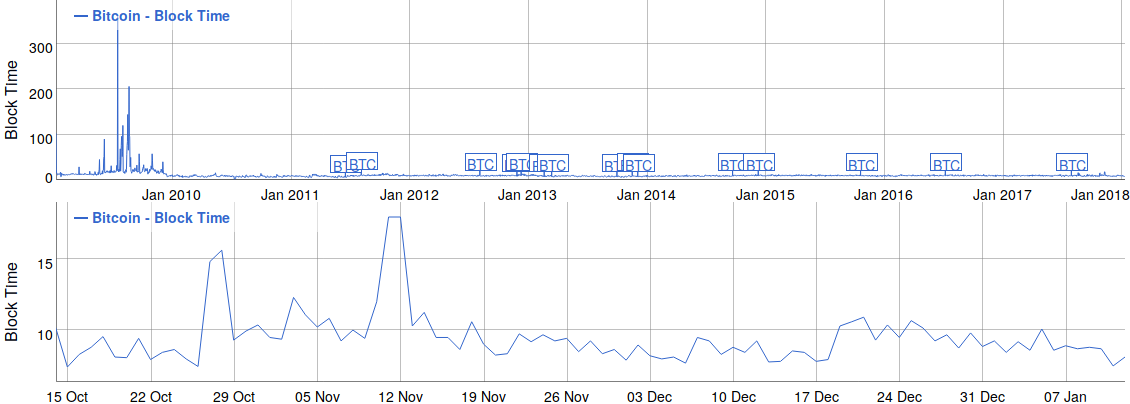
\includegraphics[width=\textwidth]{img/bitinfocharts-blocktime-btc}
%~ \caption[blocktime-btc]{\label{blocktime-btc}\mbox{Blockzeit f. Bitcoin}, \mbox{oben: Gesamt}, \mbox{unten: 6~Monate} %
%~ \mbox{Quelle: \cite{w:bitinfocharts}}
%~ } %\footnote{\url{https://bitinfocharts.com/comparison/bitcoin-confirmationtime.html}}
%~ \end{figure}

%~ Am Bsp. Bitcoin Abb.\,\ref{blocktime-btc} ist neben der Anfangsphase mit wenigen Teilnehmern eine stetige Schwankung über die Gesamte Laufzeit erkennenbar.

%~ Hierzur ist  zu sagen, dass eine größere Schwankung die geringere Wertung nach sich zieht,
%~ allerdingdings können die 

%~ \begin{figure}
%~ 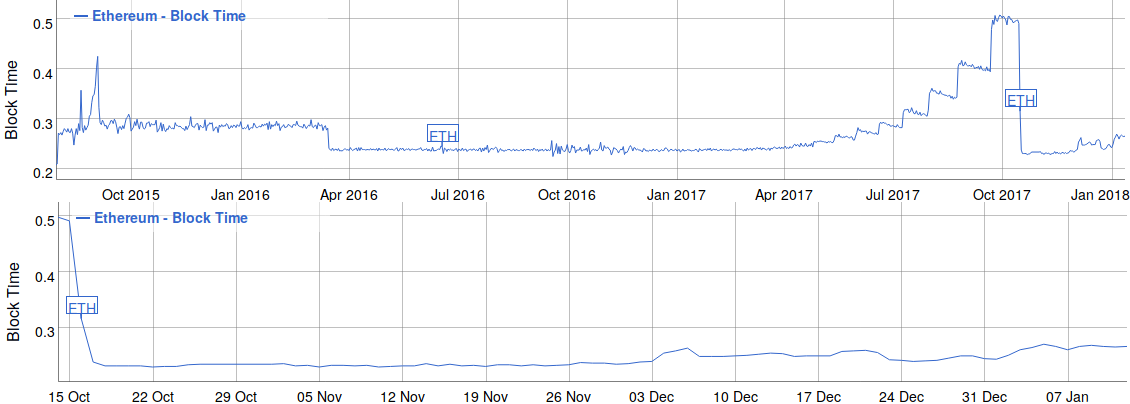
\includegraphics[width=\textwidth]{img/bitinfocharts-blocktime-eth}
%~ \caption[blocktime-eth]{\label{blocktime-eth}\mbox{Blockzeit f. Ethereum}, \mbox{oben: Gesamt}, \mbox{unten: 6~Monate} %
%~ \mbox{Quelle: \cite{w:bitinfocharts}}
%~ } %\footnote{\url{https://bitinfocharts.com/comparison/bitcoin-confirmationtime.html}}
%~ \end{figure}

%~ Bei Ethereum Abb.\,\ref{blocktime-eth} tritt eine ähnliche Auffälligkeit zur Anfangsphase auf.
%~ Zusätzlich sind sehr Deutlich Auswirkungen im März~2016\footnote{Homestead Release am 14.\,März~2016 \autocite{w:etherchain-hardforks}} und das Einsetzen der \enquote{Schwierigkeits-Bombe} (Engl. Difficulty-Bomb) bis zum abrupten Abfall\footnote{ab April~2017 (am Graph abgelesen) bis zum Byzantium Release am 16.\, Oktober~2017 \autocite{w:etherchain-hardforks}}. Beide Änderungen stehen je mit einer \gls{glos:Hard~Fork} in Verbindung.

%\begin{figure}
%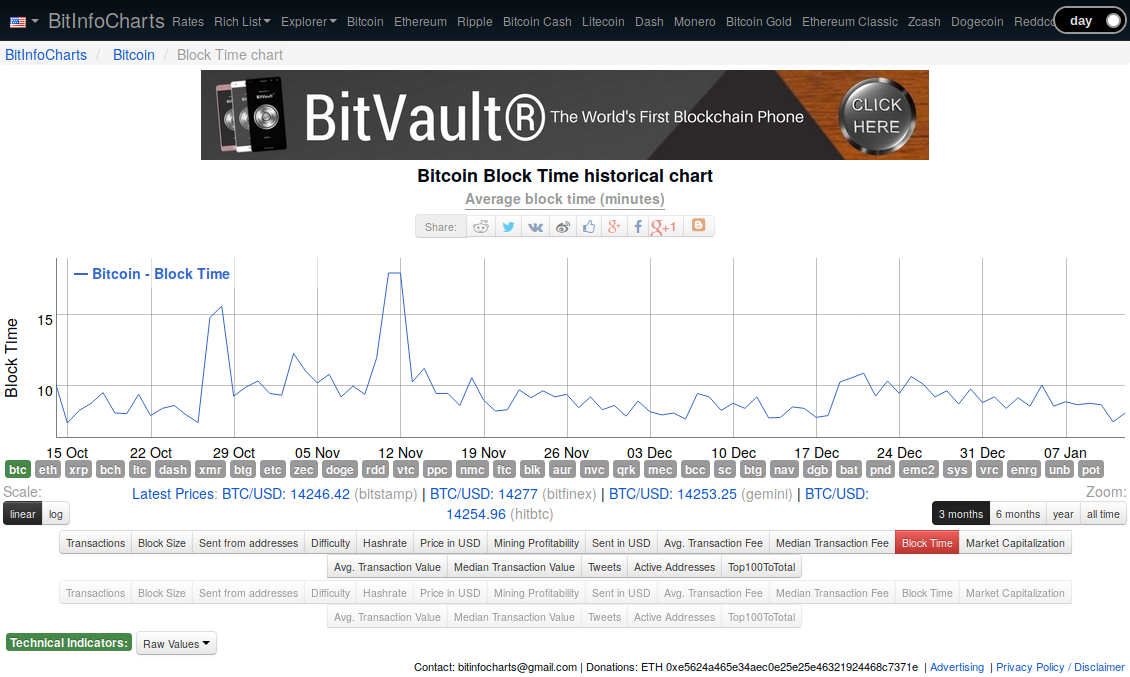
\includegraphics[width=\textwidth]{img/screenshot-bitinfocharts-2018-01-13-18-27-38}
%\end{figure}

%~ https://etherscan.io/chart/blocktime

%~ + Entwicklung von Kriterien
  %~ + Welche Eigenschaften bieten die Implementierungen
	%~ * Unterstützung
	%~ * Entwicklungsstand
	%~ * Kosten
	%~ * 
  %~ + Welchen Anwendungsfällen sind sie zu-/abträglich
	%~ * Viele Transaktionen
	%~ * Privatsphäre
	%~ * Integration Bestehender IT

%%
\section{Wirtschaftliche Gesichtspunkte}\label{krit:oeconomics}

Bevor naheliegende Kosten betrachtet werden, soll auch auf die Ertragsseite der Wirtschaftlichkeitsbetrachtung hingewiesen werden.
Die Bewertung ist sehr stark vom Einzelfall mit vielen Einflussfaktoren abhängig und wird daher in der Arbeit nicht als Kriterium aufgenommen.
Was Wertung von Angaben zu Kosten und Erträgen angeht, so sind höhere Kosten immer schlechter zu werten und höhere Erträge besser.

\subsection{Personalverfügbarkeit}\label{krit:personal}

Noch heute erscheint die Neuerung durch die \gls{BCT} so groß, dass der Bedarf an Personal nicht gedeckt ist.
%Aber ähnlich die Geometrie sind die Kenntnisse dahinter nur auf Zeit Spezialwissen.
Umso mehr Anwendungen den Alltag beeinflussen, umso mehr Informationen öffentlich zugänglich sind, desto leichter wird es sein diese Kompetenzen am Markt zu erhalten.
Bisweilen haben Firmen aber genau das Problem ihren Bedarf am Markt zu decken.

Die Betrachtung stellt auf die Verfügbarkeit von Personal und damit die Durchführbarkeit beabsichtigter Projekte ab und beinhaltet noch nicht die Kosten. 
%~ Daher spielt der Faktor Personal noch eine enorme Rolle bei initialen (horizontale Weiterbildung) und vor allem laufenden Kosten für Gehälter.
Die Wertung für geringere Personalverfügbarkeit ist kleiner als die höherer.

\subsection{Beschaffungskosten}\label{kosten}

%~ (gewonnen aus \nameref{first:kosten})
Für die Verwendung im konkreten Unternehmen notwendigen Einmalaufwendungen können eine wesentliche Zugangshürde zu Technologie darstellen.
Dies kann auch trotz \emph{offener Standards} und Open~Source Software der Fall sein wenn einzelne Akteure ihre Position oder ihren Wissensvorsprung monetarisieren.
Initiale Kosten können insbesondere Anschaffung von Hardware und ggf. Lizenzkosten\footnote{Bsp. Softwarelizenzen, Nutzungslizenz für Patente; auch Konzessionen wie die \emph{BitLicense} \autocite{w:bitlicense}} darstellen.
Auch andere Einmalaufwendungen -- \zB{} für den Zugang zu Verbänden -- zählen hierzu.

BigchainDB hat keine Preisliste, ist aber gesprächsbereit sofern Interesse an Beratung besteht.
Bei Hyperledger ist die intensive Mitarbeit für gewinnorientierte Unternehmen Gebührenpflichtig.
Gemeinnützige Organisationen können sich für eine kostenlose Mitgliedschaft bewerben.

\subsection{Laufende Kosten}

Abgesetzt von den Beschaffungskosten sind auch laufende Kosten zu betrachten.
Hier insbesondere Beiträge zu Verbänden und auf die \gls{BCI} beziehbare Personalkosten (s.a. \ref{krit:personal}) wie Gehälter und Weiterbildung.

%~ (gewonnen aus \nameref{first:regulierung})
Abgesehen von den Kosten ist auch die Beeinflussung des Umfeldes durch
Standardisierung und Regulierung (\label{regulierung}s. \ref{first:regulierung}) für Unternehmen eine Herausforderung.
Dabei können Kosten unregelmäßig auftreten und unvorhersehbar auftreten.

\subsection{Organisation}

Die Wirtschaftliche Organisation ist vergleichbar mit der \nameref{krit:community} (\ref{krit:community}).
Auch auf der Ebene der Betreiber soll eine Absicherung nicht vernachlässigt werden.
Ähnlich einem zentralen Entwickler kann eine zentrale Organisation ein Risiko für das Vertrauen darstellen.
Üblich sind inzwischen gemeinnützige Stiftungen, die die Weiterentwicklung einer Implementation und des Ökosystems darum sicherstellen sollen.
Diese ermöglichen auch eine Beteiligung weiterer -- natürlicher wie juristischer -- Personen.

Eine gemeinnützige Organisationsform ist ggü. einer gewinnorientierten hinsichtlich des in sie gesetzten Vertrauens besser zu werten.
Teilnahme-/Zugangsbeschränkung und Gleichheit können innerhalb einer solchen Organisation als zusätzliche Wertungsmöglichkeit herangezogen werden.
